\subsection{Confronto test salvati}

\begin{figure}[H]
    \centering
    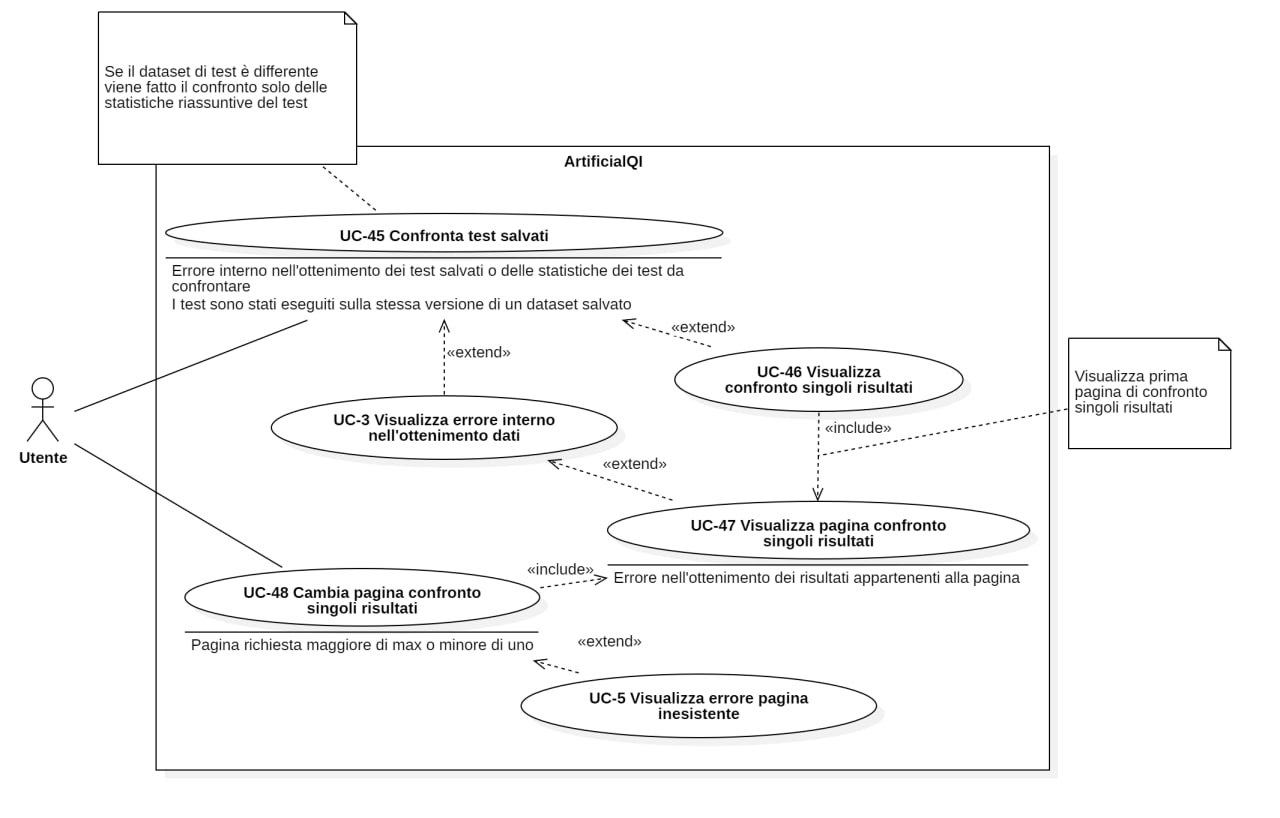
\includegraphics[scale=0.45]{Sezioni/UseCase/Immagini/ConfrontoTest.png}
    \caption{Diagramma per il confronto di test salvati.}
\end{figure}

\begin{usecase}{UC-45}{Confronta test salvati}
    \label{uc:UC-45}
    
    \req{\hyperref[ru:RUF-5]{RUF-5}}
    
    \pre{
        \item L'utente sta visualizzando i risultati del test caricato
        \item Il test caricato condivide il dataset e/o l'LLM utilizzati nel test con almeno un altro test salvato
    }
    
    \post{
        \item L'utente visualizza il confronto tra il test caricato e un test salvato
    }
    
    \actor{
        Utente
    }
    
    \subactors{}
    
    \trigger{L'utente vuole confrontare il test caricato con un test salvato}
    
    \inc{}
    
    \base{}
    
    \scenario{
        \item L'utente richiede l'esecuzione di un confronto con il test caricato
        \item Il sistema richiede la selezione di un test salvato tra quelli che condividono dataset e/o LLM con il test caricato
        \item Il sistema ottiene le statistiche riassuntive del test selezionato
        \item L'utente visualizza i due indici riassuntivi dei test a confronto 
        \item Il sistema verifica che i due test confrontati non siano stati eseguiti sulla stessa versione del dataset
    }
    
    \subscenario{
        \item[2.1]Avviene un errore interno durante l'ottenimento dei test salvati confrontabili con il test caricato:
        \begin{itemize}
            \item \hyperref[uc:UC-3]{UC-3}
        \end{itemize}
        \item[3.1] Avviene un errore interno durante l'ottenimento delle statistiche del test:
        \begin{itemize}
            \item \hyperref[uc:UC-3]{UC-3}
        \end{itemize}
        \item[5.1] I test sono stati eseguiti sulla stessa versione di uno stesso dataset:
        \begin{itemize}
            \item \hyperref[uc:UC-46]{UC-46}
        \end{itemize}
    }

\end{usecase}


\begin{usecase}{UC-46}{Visualizza confronti singoli risultati}
    \label{uc:UC-46}
    
    \req{}
    
    \pre{
        \item I due test coinvolti nel confronto sono stati eseguiti sulla stessa versione dello stesso dataset 
    }
    
    \post{
        \item Vengono visualizzati i confronti dei singoli risultati dei due test
    }
    
    \actor{
        Utente
    }
    
    \subactors{}
    
    \trigger{L'utente ha richiesto il confronto tra due test eseguiti sullo stessa versione dello stesso dataset}
    
    \inc{\hyperref[uc:UC-47]{UC-47}}
    
    \base{}
    
    \scenario{
        \item Il sistema visualizza la prima pagina di risultati seguendo \hyperref[uc:UC-47]{UC-47}
    }
    
    \subscenario{}

\end{usecase}

\begin{usecase}{UC-47}{Visualizza pagina confronto singoli risultati}
    \label{uc:UC-47}
    
    \req{}
    
    \pre{
        \item La pagina da visualizzare esiste
    }
    
    \post{
        \item Vengono visualizzati i confronti dei singoli risultati dei due test appartenenti alla pagina richiesta
    }
    
    \actor{}
    
    \subactors{}
    
    \trigger{Il sistema deve visualizzare una pagina contenente i confronti tra i singoli risultati di due test}
    
    \inc{}
    
    \base{}
    
    \scenario{
        \item Il sistema ottiene i risultati che appartengono alla pagina richiesta
        \item Il sistema mostra il diagramma di dispersione contenente sotto forma di coppie di punti i risultati a confronto che appartengono alla pagina richiesta
        \item Il sistema mostra il confronto tra le coppie di risultati in una lista 
    }
    
    \subscenario{
        \item[1.1] Il sistema riscontra un errore interno durante l'ottenimento dei risultati appartenenti alla pagina richiesta:
        \begin{itemize}
            \item \hyperref[uc:UC-3]{UC-3}
        \end{itemize}
    }

\end{usecase}

\begin{usecase}{UC-48}{Cambia pagina confronto singoli risultati}
    \label{uc:UC-48}
    
    \req{}
    
    \pre{
        \item L'utente sta visualizzando il confronto dei singoli risultati di una coppia di test
    }
    
    \post{
        \item Viene visualizzata la pagina richiesta
    }
    
    \actor{Utente}
    
    \subactors{}
    
    \trigger{L'utente vuole visualizzare una specifica pagina di confronto tra i singoli risultati}
    
    \inc{\hyperref[uc:UC-47]{UC-47}}
    
    \base{}
    
    \scenario{
        \item Il sistema verifica che la pagina sia valida
        \item Viene visualizzata la pagina richiesta seguendo \hyperref[uc:UC-47]{UC-47}
    }
    
    \subscenario{
        \item[2.1] La pagina richiesta non è valida ovvero è inferiore a uno o superiore alla pagina massima:
        \begin{itemize}
            \item \hyperref[uc:UC-2]{UC-2}
        \end{itemize}
    }

\end{usecase}